\documentclass[11pt,a4paper]{article}

% Packages
\usepackage[utf8]{inputenc}
\usepackage[T1]{fontenc}
\usepackage{amsmath,amssymb,amsthm}
\usepackage{physics}
\usepackage{graphicx}
\usepackage{hyperref}
\usepackage{geometry}
\usepackage{enumitem}
\usepackage{fancyhdr}
\usepackage{tcolorbox}
\usepackage{tikz}
\usepackage{microtype}
\usepackage{needspace}
\usetikzlibrary{arrows.meta,decorations.pathmorphing}

% Compact lists
\setlist{nosep}

% Prevent orphaned headings
\let\oldsection\section
\renewcommand{\section}{\needspace{5\baselineskip}\oldsection}
\let\oldsubsection\subsection
\renewcommand{\subsection}{\needspace{4\baselineskip}\oldsubsection}
\let\oldsubsubsection\subsubsection
\renewcommand{\subsubsection}{\needspace{3\baselineskip}\oldsubsubsection}

\geometry{margin=2.5cm}
\setlength{\headheight}{14pt}

% Theorem environments
\theoremstyle{definition}
\newtheorem{definition}{Definition}[section]
\newtheorem{example}{Example}[section]
\theoremstyle{remark}
\newtheorem{remark}{Remark}[section]

% Box environments
\newtcolorbox{keyresult}{
    colback=blue!5!white,
    colframe=blue!75!black,
    title=Key Result
}

\newtcolorbox{insight}{
    colback=green!5!white,
    colframe=green!50!black,
    title=Physical Insight
}

% Header
\pagestyle{fancy}
\fancyhf{}
\rhead{Ali EL AZDI -- BA5}
\lhead{Quantum Motion in a Magnetic Field}
\cfoot{\thepage}

\title{\textbf{Quantum Motion in a Uniform Magnetic Field}}
\author{Ali EL AZDI \\ BA5}
\date{January 2026}

\begin{document}

\maketitle

\begin{abstract}
This document explains how an electron moves in a magnetic field when we use quantum mechanics instead of classical physics. We will see that the electron can only have certain specific energies, called \textbf{Landau levels}. The document starts from the basics, so you don't need to know quantum mechanics beforehand---just some calculus and linear algebra.
\end{abstract}
\newpage
\tableofcontents
\newpage

%==============================================================================
\section{Why Study This Problem?}
%==============================================================================

Charged particles in magnetic fields are everywhere in physics, but studying this specific problem reveals deep quantum phenomena:
\begin{itemize}
    \item \textbf{Theoretical Foundation}: It is one of the few exactly solvable interactions in Quantum Mechanics.
    \item \textbf{Condensed Matter}: It describes electrons in metals and semiconductors, particularly the 2D electron gas (2DEG).
    \item \textbf{Quantum Hall Effect}: It explains macroscopic quantum phenomena and currently defines our electrical resistance standards.
\end{itemize}

At large scales, classical physics works well. But when we look at electrons in materials at very low temperatures and strong magnetic fields, quantum effects take over. This leads to amazing things like the \textbf{Quantum Hall Effect}, which won the Nobel Prize in 1985.

In this document, we answer one question:

\begin{center}
\textit{What energies can an electron have when it moves in a uniform magnetic field?}
\end{center}

The answer is surprising: the energy is \textbf{quantized}---only certain values are allowed.

%==============================================================================
\section{Background: What You Need to Know}
%==============================================================================

Let's first review the classical physics and learn the quantum mechanics basics we need.

%------------------------------------------------------------------------------
\subsection{Classical Motion in a Magnetic Field}
%------------------------------------------------------------------------------

A particle with charge $q$ moving at velocity $\vec{v}$ in an electromagnetic field is subject to the general \textbf{Lorentz force}:
\begin{equation}
    \vec{F} = q(\vec{E} + \vec{v} \times \vec{B})
\end{equation}
Since the magnetic field is static ($\frac{\partial \vec{B}}{\partial t} = \vec{0}$), there are no induced electric fields. Assuming no external electric field is applied ($\vec{E} = \vec{0}$), the force simplifies to:
\begin{equation}
    \vec{F} = q\vec{v} \times \vec{B}
\end{equation}

In our visualization, we model the following specific setup:
\begin{itemize}
    \item[-] \textbf{System:} A negatively charged particle ($q < 0$) confined to the $xy$-plane.
    \item[-] \textbf{Field:} A \textbf{static, uniform, external} magnetic field $\vec{B} = B\hat{z}$ pointing out of the page. It is constant in time \textbf{(no induced electric fields)} and we neglect the particle's self-field.
    \item[-] \textbf{Motion:} The Lorentz force acts as a pure centripetal force, resulting in \textbf{counter-clockwise uniform circular motion}.
\end{itemize}

The radius and frequency of this orbit are given by:
\begin{align}
    r &= \frac{mv}{|q|B} \quad \text{(cyclotron radius)} \\
    \omega_c &= \frac{|q|B}{m} \quad \text{(cyclotron frequency)}
\end{align}

\begin{remark}
In classical mechanics, the radius $r$ (and thus the energy) can be any continuous value. Quantum mechanics will restrict this to discrete levels.
\end{remark}

%------------------------------------------------------------------------------
\subsection{The Vector Potential}
%------------------------------------------------------------------------------

Since the magnetic field is always divergence-free ($\nabla \cdot \vec{B} = 0$), it can be expressed as the curl of a \textbf{vector potential} $\vec{A}$:
\begin{equation}
    \vec{B} = \nabla \times \vec{A}
\end{equation}

The choice of $\vec{A}$ is not unique. We can add the gradient of any scalar function $\chi$ to the potential without changing the physical magnetic field. This is known as \textbf{gauge freedom}.
\begin{equation}
    \vec{A}' = \vec{A} + \nabla\chi
\end{equation}

This transformation leaves $\vec{B}$ invariant because the curl of a gradient is identically zero ($\nabla \times (\nabla \chi) = 0$):
\begin{equation}
    \vec{B}' = \nabla \times \vec{A}' = \nabla \times \vec{A} + \underbrace{\nabla \times (\nabla\chi)}_{0} = \vec{B}
\end{equation}

For a uniform field $\vec{B} = B\hat{z}$, we choose the \textbf{Landau gauge}:
\begin{equation}
    \vec{A} = (0, Bx, 0) = Bx\hat{y}
\end{equation}
We verify this choice by explicitly calculating the curl:
\begin{equation}
    \nabla \times \vec{A} = \left( \frac{\partial A_y}{\partial x} - \frac{\partial A_x}{\partial y} \right) \hat{z} = \left( \frac{\partial (Bx)}{\partial x} - 0 \right) \hat{z} = B\hat{z}
\end{equation}



%==============================================================================
\section{Setting Up the Problem}
%==============================================================================

We can now construct the Hamiltonian for our specific problem by applying the correspondence principle to the classical description.

%------------------------------------------------------------------------------
\subsection{Deriving the Classical Hamiltonian}
%------------------------------------------------------------------------------

We can derive the Hamiltonian by expressing the total energy in terms of the correct canonical variables, without needing the full Lagrangian formalism.

\subsubsection{Step 1: The Total Energy}
The magnetic force $\vec{F}_B = q(\vec{v} \times \vec{B})$ is always perpendicular to the velocity, so it does no work on the particle. Therefore, the magnetic field does not add a scalar potential energy term. The total energy is simply the kinetic energy plus the potential energy from any electric field $\phi$:
\begin{equation}
    E_{total} = \frac{1}{2}m\vec{v}^2 + q\phi
\end{equation}

\subsubsection{Step 2: Canonical Momentum}
Hamiltonian mechanics requires us to express system dynamics in terms of position $\vec{r}$ and \textbf{canonical momentum} $\vec{p}$. In the presence of a magnetic field, the momentum variable that satisfies Hamilton's canonical equations is not just $m\vec{v}$, but includes a field term:
\begin{equation}
    \vec{p} = m\vec{v} + q\vec{A}
\end{equation}
\textit{Justification:} One can verify that using this definition in Hamilton's equations ($\dot{\vec{p}} = -\nabla H$, $\dot{\vec{r}} = \nabla_p H$) correctly reproduces the Lorentz force law $\vec{F} = q(\vec{E} + \vec{v} \times \vec{B})$.

\subsubsection{Step 3: Constructing the Hamiltonian}
The Hamiltonian is the total energy expressed in terms of $\vec{r}$ and $\vec{p}$.
From Step 2, we rearrange to find velocity: $\vec{v} = \frac{1}{m}(\vec{p} - q\vec{A})$.
Substituting this into the energy equation from Step 1:
\begin{equation}
    H(\vec{r}, \vec{p}) = \frac{1}{2}m \left( \frac{\vec{p} - q\vec{A}}{m} \right)^2 + q\phi = \frac{1}{2m}(\vec{p} - q\vec{A})^2 + q\phi
\end{equation}

Note that this Hamiltonian depends on the vector potential $\vec{A}$, which is defined only up to a gauge transformation. To explicitly solve for the motion, we will eventually need to make a specific gauge choice.

%------------------------------------------------------------------------------
\subsection{Quick Introduction to Quantum Mechanics}
%------------------------------------------------------------------------------

To treat this problem quantum mechanically, we rely on the fundamental postulates of the theory.

\subsubsection{The State of the System}

In quantum mechanics, the state of a particle is completely described by a wave function $\psi(\vec{r}, t)$, which resides in a Hilbert space of square-integrable functions. The physical interpretation is probabilistic:
\begin{equation}
    P(\vec{r}) = |\psi(\vec{r}, t)|^2
\end{equation}
is the probability density of finding the particle at position $\vec{r}$.

\subsubsection{Observables as Operators}

Every physical observable corresponds to a linear Hermitian operator acting on the wave function. The fundamental operators are:
\begin{itemize}
    \item \textbf{Position operator:} $\hat{\vec{r}} \psi = \vec{r} \psi$ (multiplication by position)
    \item \textbf{Momentum operator:} $\hat{\vec{p}} \psi = -i\hbar\nabla \psi$ (differentiation)
\end{itemize}
These operators satisfy the canonical commutation relation:
\begin{equation}
    [\hat{x}, \hat{p}_x] = \hat{x}\hat{p}_x - \hat{p}_x\hat{x} = i\hbar
\end{equation}
where $\hbar \approx 1.05 \times 10^{-34}$ J$\cdot$s is the reduced Planck constant.

\subsubsection{The Schrödinger Equation}

The dynamics of the system are governed by the Schrödinger equation. For stationary states (states with definite energy $E$), it takes the time-independent form:
\begin{equation}
    \hat{H}\psi(\vec{r}) = E\psi(\vec{r})
\end{equation}
Here, $\hat{H}$ is the \textbf{Hamiltonian operator}, which corresponds to the total energy of the system.

%------------------------------------------------------------------------------
\subsection{The Quantum Formulation}
%------------------------------------------------------------------------------

We obtain the quantum theory by promoting the classical canonical variables to operators (canonical quantization):
\begin{equation}
    \vec{r} \to \hat{\vec{r}}, \quad \vec{p} \to \hat{\vec{p}} = -i\hbar\nabla
\end{equation}

Substituting these into the general classical Hamiltonian yields the \textbf{general quantum Hamiltonian}:
\begin{equation}
    \hat{H} = \frac{1}{2m}\left(\hat{\vec{p}} - q\vec{A}(\hat{\vec{r}})\right)^2 + q\phi(\hat{\vec{r}})
\end{equation}

Now we specify our physical system and make a gauge choice to find the explicit differential equation:
\begin{enumerate}
    \item \textbf{Particle:} Charged particle with charge $q$.
    \item \textbf{Potentials:} No electric field ($\phi = 0$).
    \item \textbf{Gauge Choice:} We select the \textbf{Landau gauge} $\vec{A} = (0, Bx, 0)$ to represent the uniform field $\vec{B} = B\hat{z}$.
\end{enumerate}

Plugging these into the general operator:
\begin{equation}
    \hat{H} = \frac{1}{2m}\left[ \hat{p}_x^2 + (\hat{p}_y - qBx)^2 + \hat{p}_z^2 \right]
\end{equation}

The time-independent Schrödinger equation $\hat{H}\psi = E\psi$ becomes:
\begin{equation}
    \frac{1}{2m}\left[ -\hbar^2\frac{\partial^2}{\partial x^2} + \left(-i\hbar\frac{\partial}{\partial y} - qBx\right)^2 - \hbar^2\frac{\partial^2}{\partial z^2} \right] \psi(x,y,z) = E\psi(x,y,z)
\end{equation}

This is the differential equation we must solve to find the energy spectrum.

%==============================================================================
\section{Solving the Equation}
%==============================================================================

%------------------------------------------------------------------------------
\subsection{Separation of Variables}
%------------------------------------------------------------------------------

Since $\hat{H}$ does not depend on $y$ or $z$, the momenta $p_y$ and $p_z$ are conserved. We can write the wave function as:
\begin{equation}
    \psi(x, y, z) = e^{ik_y y} \cdot e^{ik_z z} \cdot \phi(x)
\end{equation}

Here $k_y$ and $k_z$ are constants (wave numbers). When $\hat{p}_y$ acts on this:
\begin{equation}
    \hat{p}_y \psi = \hbar k_y \psi
\end{equation}

So $\hbar k_y$ is the momentum in the $y$-direction, and $\hbar k_z$ is the momentum in the $z$-direction.

%------------------------------------------------------------------------------
\subsection{Reducing to One Dimension}
%------------------------------------------------------------------------------

Putting our wave function into the Schrödinger equation and simplifying:
\begin{equation}
    \left[\frac{\hat{p}_x^2}{2m} + \frac{(\hbar k_y - qBx)^2}{2m}\right]\phi(x) = \left(E - \frac{\hbar^2 k_z^2}{2m}\right)\phi(x)
\end{equation}

The $z$-motion just gives free particle kinetic energy $\frac{\hbar^2 k_z^2}{2m}$. The interesting physics is in the $xy$-plane.

%------------------------------------------------------------------------------
\subsection{Finding the Hidden Harmonic Oscillator}
%------------------------------------------------------------------------------

Let's define a \textbf{center position}:
\begin{equation}
    x_0 = \frac{\hbar k_y}{qB}
\end{equation}

Then we can rewrite:
\begin{equation}
    \hbar k_y - qBx = -qB(x - x_0)
\end{equation}

The equation becomes:
\begin{equation}
    \left[\frac{\hat{p}_x^2}{2m} + \frac{(qB)^2(x - x_0)^2}{2m}\right]\phi(x) = \left(E - \frac{\hbar^2 k_z^2}{2m}\right) \phi(x)
\end{equation}

Using $\omega_c = |q|B/m$, we can write $(qB)^2/(2m) = m\omega_c^2/2$. So:
\begin{equation}
    \boxed{\left[\frac{\hat{p}_x^2}{2m} + \frac{1}{2}m\omega_c^2(x - x_0)^2\right]\phi(x) = \left(E - \frac{\hbar^2 k_z^2}{2m}\right) \phi(x)}
\end{equation}

\begin{keyresult}
This is exactly a \textbf{harmonic oscillator} centered at $x_0$ with frequency $\omega_c$! The magnetic field creates an effective spring potential.
\end{keyresult}

%==============================================================================
\section{The Results: Landau Levels}
%==============================================================================

%------------------------------------------------------------------------------
\subsection{The Energy Spectrum}
%------------------------------------------------------------------------------

Since the $x$-motion is a harmonic oscillator, the energies are:
\begin{equation}
    E - \frac{\hbar^2 k_z^2}{2m} = \hbar\omega_c\left(n + \frac{1}{2}\right), \quad n = 0, 1, 2, \ldots
\end{equation}

Adding back the kinetic energy from motion along $z$:
\begin{keyresult}
The full energy spectrum is:
\begin{equation}
    \boxed{E_{n, k_z} = \hbar\omega_c\left(n + \frac{1}{2}\right) + \frac{\hbar^2 k_z^2}{2m}}
\end{equation}
These discrete energy levels are called \textbf{Landau levels}.
\end{keyresult}

\begin{center}
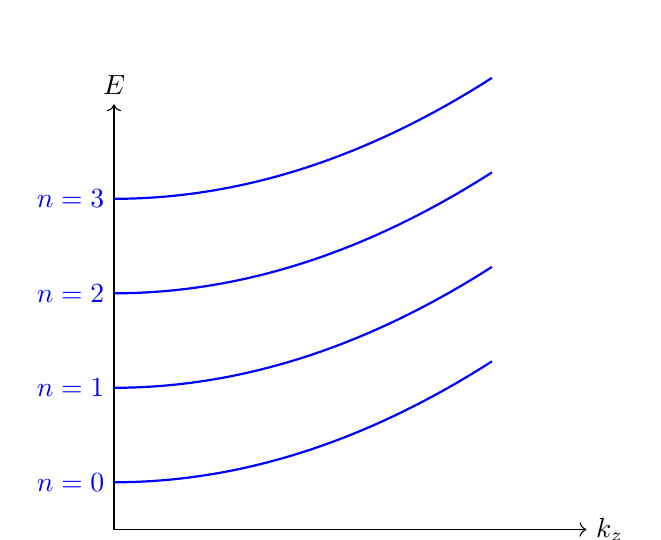
\begin{tikzpicture}[scale=1.2]
    % Axes
    \draw[->] (0,0) -- (5,0) node[right] {$k_z$};
    \draw[->] (0,0) -- (0,4.5) node[above] {$E$};
    
    % Landau levels
    \foreach \n/\label in {0.5/$n=0$, 1.5/$n=1$, 2.5/$n=2$, 3.5/$n=3$} {
        \draw[thick, blue] plot[domain=0:4, samples=50] (\x, {\n + 0.08*\x*\x});
        \node[left, blue] at (0, \n) {\label};
    }
\end{tikzpicture}
\end{center}

%------------------------------------------------------------------------------
\subsection{What Does This Mean Physically?}
%------------------------------------------------------------------------------

\begin{insight}
\begin{itemize}
    \item The quantum number $n$ labels the different Landau levels
    \item Higher $n$ means higher energy (like climbing a ladder)
    \item The spacing between levels is $\hbar\omega_c$---bigger for stronger magnetic fields
    \item Motion along $z$ (parallel to $\vec{B}$) is still free---any $k_z$ is allowed
    \item Motion in the $xy$-plane is quantized (only specific orbits allowed)
\end{itemize}
\end{insight}

\begin{example}[Typical Numbers]
For an electron in a 10 Tesla field:
\begin{align}
    \omega_c &= \frac{|q|B}{m} \approx 1.76 \times 10^{12} \text{ rad/s} \\
    \hbar\omega_c &\approx 1.2 \text{ meV} \approx 13 \text{ K (in temperature units)}
\end{align}
To see Landau levels clearly, we need temperatures below about 4 K and strong magnetic fields.
\end{example}

%------------------------------------------------------------------------------
\subsection{The Wave Functions}
%------------------------------------------------------------------------------

The complete wave function is:
\begin{equation}
    \psi_{n, k_y, k_z}(x, y, z) = e^{ik_y y} \cdot e^{ik_z z} \cdot \phi_n(x - x_0)
\end{equation}

where $\phi_n$ are the standard harmonic oscillator wave functions (involving Hermite polynomials).

\begin{insight}
What does this wave function look like?
\begin{itemize}
    \item Localized in $x$ around the center $x_0 = \hbar k_y/(qB)$
    \item Spread uniformly in $y$ (plane wave)
    \item Different degenerate states have different centers $x_0$
\end{itemize}
Think of it as cyclotron orbits at different positions across the sample, all with the same energy.
\end{insight}

%------------------------------------------------------------------------------
\subsection{Degeneracy: Many States with the Same Energy}
%------------------------------------------------------------------------------

Look at the energy formula: it depends on $n$ and $k_z$, but \textbf{not on $k_y$}. Different values of $k_y$ give different states but the same energy. This is called \textbf{degeneracy}.

To find the number of states $N$ in a sample of area $A = L_x \times L_y$, we count the allowed values of $k_y$:

\begin{enumerate}
    \item The oscillator center $x_0 = \frac{\hbar k_y}{qB}$ must be inside the sample ($0 \le x_0 \le L_x$). This restricts the range of allowed momentum:
    \begin{equation}
        \Delta k_y = \frac{|q|B}{\hbar} \Delta x_0 = \frac{|q|B L_x}{\hbar}
    \end{equation}
    \item Periodic boundary conditions along $y$ require $k_y = \frac{2\pi n}{L_y}$, so the spacing between states is $\delta k_y = \frac{2\pi}{L_y}$.
    \item The total number of states is the range divided by the spacing:
    \begin{equation}
        N = \frac{\Delta k_y}{\delta k_y} = \frac{|q|B L_x}{\hbar} \cdot \frac{L_y}{2\pi} = \frac{|q|B (L_x L_y)}{h}
    \end{equation}
\end{enumerate}

Thus, the degeneracy is:
\begin{equation}
    N = \frac{|q|BA}{h} = \frac{\Phi}{\Phi_0}
\end{equation}

where $\Phi = BA$ is the total magnetic flux and $\Phi_0 = h/|q| \approx 4.14 \times 10^{-15} \text{ Wb}$ is the \textbf{flux quantum}.

\begin{keyresult}
The degeneracy of each Landau level equals the number of flux quanta through the sample:
\begin{equation}
    \boxed{N = \frac{\text{Magnetic flux}}{\text{Flux quantum}} = \frac{BA}{h/|q|}}
\end{equation}
\end{keyresult}

\begin{example}[How Large is the Degeneracy?]
For a 1 cm $\times$ 1 cm sample in a 1.5 T field (typical MRI):
\begin{equation}
    N = \frac{(1.6 \times 10^{-19})(1.5)(10^{-4})}{6.63 \times 10^{-34}} \approx 3.6 \times 10^{10}
\end{equation}
Each Landau level has about 36 billion states! This huge degeneracy is key to the Quantum Hall Effect.
\end{example}

%------------------------------------------------------------------------------
\subsection{Physical Scale: The Magnetic Length}
%------------------------------------------------------------------------------

We encountered a harmonic oscillator frequency $\omega_c = |q|B/m$. The harmonic oscillator also has a characteristic length scale, $x_{osc} = \sqrt{\frac{\hbar}{m\omega}}$. Substituting $\omega_c$, we get the \textbf{magnetic length}:

\begin{equation}
    \ell_B = \sqrt{\frac{\hbar}{m\omega_c}} = \sqrt{\frac{\hbar}{m\left(\frac{|q|B}{m}\right)}} = \sqrt{\frac{\hbar}{|q|B}}
\end{equation}

This length scale defines the spread of the wave function in the $xy$-plane.

\begin{example}[Estimating the Magnetic Length]
For our example with $B = 1.5\,\text{T}$:
\begin{equation}
    \ell_B = \sqrt{\frac{1.055 \times 10^{-34}}{1.6 \times 10^{-19} \times 1.5}} \approx 2.1 \times 10^{-8}\,\text{m} = 21\,\text{nm}
\end{equation}
\end{example}

\begin{insight}
\textbf{Physical Significance:}
\begin{itemize}
    \item $\ell_B$ sets the characteristic size of the electron's orbit (wavefunction) in the magnetic field.
    \item The area occupied by one quantum state is approximately $2\pi\ell_B^2$.
    \item As $B$ increases, $\ell_B$ decreases, meaning the electrons are more tightly confined (stronger localization), which enhances quantum effects.
\end{itemize}
\end{insight}

%==============================================================================
\section{Why This Matters: Modern Applications}
%==============================================================================

%------------------------------------------------------------------------------
\subsection{The Quantum Hall Effect}
%------------------------------------------------------------------------------

 In a thin layer of electrons at low temperature and high magnetic field, the electrical resistance is quantized:
\begin{equation}
    R_{xy} = \frac{h}{ne^2}, \quad n = 1, 2, 3, \ldots
\end{equation}

This is incredibly precise (better than 1 part in a billion!) and is now used as the international standard for electrical resistance. It happens because of Landau level quantization.

%------------------------------------------------------------------------------
\subsection{Graphene}
%------------------------------------------------------------------------------

In graphene (a single layer of carbon atoms), electrons behave differently. The Landau levels follow:
\begin{equation}
    E_n = \pm v_F \sqrt{2eB\hbar n}
\end{equation}
The $\sqrt{n}$ dependence (instead of $n$) and the zero-energy level at $n=0$ are signs that electrons in graphene act like relativistic particles.

%==============================================================================
\section{Summary}
%==============================================================================

\begin{keyresult}
\textbf{What We Learned:}

\begin{enumerate}
    \item An electron in a uniform magnetic field has \textbf{quantized energies} called Landau levels:
    \begin{equation}
        E_n = \hbar\omega_c\left(n + \frac{1}{2}\right), \quad \omega_c = \frac{|q|B}{m}
    \end{equation}
    
    \item Each level is highly \textbf{degenerate}---many states share the same energy:
    \begin{equation}
        N = \frac{|q|BA}{h}
    \end{equation}
    
    \item The natural length scale is the \textbf{magnetic length}:
    \begin{equation}
        \ell_B = \sqrt{\frac{\hbar}{|q|B}}
    \end{equation}
    
    \item The problem reduces to a \textbf{harmonic oscillator}---that's why the energy is quantized.
\end{enumerate}
\end{keyresult}

\begin{insight}
\textbf{The Big Picture:}

Landau levels are the foundation for:
\begin{itemize}
    \item The Quantum Hall Effect (used to define the unit of resistance)
    \item Studying electronic properties of metals
    \item Understanding new materials like graphene
    \item Modern research on topological phases of matter
\end{itemize}
\end{insight}

%==============================================================================
\appendix
\section{Gauge Invariance}
%==============================================================================

You might wonder: if we pick a different vector potential $\vec{A}$, do we get different physics?

The answer is \textbf{no}. Different gauges give different-looking wave functions, but all measurable quantities (energies, probabilities, etc.) stay the same.

If we change the gauge:
\begin{equation}
    \vec{A} \to \vec{A}' = \vec{A} + \nabla\chi
\end{equation}
the wave function changes by a phase factor:
\begin{equation}
    \psi \to \psi' = e^{iq\chi/\hbar} \psi
\end{equation}
This phase cancels out in any physical measurement.
\\
%==============================================================================
\section{Including Spin}
%==============================================================================

Electrons have an intrinsic angular momentum called \textbf{spin}. In a magnetic field, this adds an extra energy:
\begin{equation}
    E_{\text{spin}} = \pm \frac{1}{2}g_s\mu_B B
\end{equation}
where $g_s \approx 2$ and $\mu_B = |q|\hbar/(2m)$ is the Bohr magneton.

This splits each Landau level into two:
\begin{equation}
    E_{n, \pm} = \hbar\omega_c\left(n + \frac{1}{2}\right) \pm \frac{1}{2}g_s\mu_B B
\end{equation}

For $g_s = 2$, the spin splitting equals the Landau level spacing, leading to interesting effects.

\end{document}
